
\chapter{Application}
\label{cha:application}

This chapter present two more involved cases of identification. The first case
is identification of the COST beam, introduced as a standard test case for
polynomial nonlinearities, ie. two polynomial nonlinearities at the same DOF.
The second case demonstrate the usage of cubic spines to identify a system with
two different clearances. The clearance distances are also found.


\section{COST beam}
\label{sec:cost-beam}

The European action COST F3 nonlinear beam \autocite{GOLINVAL2003} was
introduced in 2003 as a benchmark system for nonlinear vibrations. The
experimental setup is shown in fig. \ref{fig:beam_setup} and consists of a
clamped beam with a thin beam part at the end of the main beam.

\begin{figure}[!ht]
  \centering
  \includegraphics[width=1\textwidth]{nlbeam/beam_setup.png}
  \caption{Experimental setup for the COST beam. Both vertical and horizontal
    setups were tested at University Liege(ULg). Horizontal setups avoids
    gravitational effects which cannot be ignored due to static deflection of
    the thin beam.}
  \label{fig:beam_setup}
\end{figure}


Accelerations are measured evenly along the beam at seven locations and excited
at node two.
From \textcite{lenaerts2003a} is it known that the system exhibit a (geometric)
cubic nonlinearity located at the tip of the main beam. Using data given at the
Nolinsys course, the beam will be identified as an example of a multiple inputs,
multiple outputs(MIMO) system. After successful identification a FE model is
built using the identified parameters and used for further examination.

The cubic nonlinearity is described to be due to \textit{large deformation of the
  tip of the thin beam}. This is a bit vague description and could include both
large rotations and midplane stretching. As both ends are clamped, the
nonlinearity probably stems from midplane stretching of the thin beam.
In \autocite{juel2003a} it is shown how both midplane stretching and large
rotations of a beam leads to a duffing equation with a cubic hardening.

Due to the thin beam, the effect of gravity is not negligible. In a vertical
setup the static deflection at the beam tip imposes a non-negligible prestress
in the thin beam, giving a nonsymmetric restoring force. This is identified as a
quadratic nonlinearity and the effect is simply removed by using a horizontal
setup.

\subsection{Identification}

The time series were obtained from University Liege(ULg), where the beam was
built as part of the COST F3 project. Unfortunately, despite several request,
only noise-free simulated data were given and not the original experimental
data.

For characterisation the beam is excited with a sine sweep. The wavelet
transform and RFS is seen in fig. \ref{fig:nlbeam_characterisation}. From the
WT, the fundamental forcing frequency is seen along with even(2:1,4:1,...) and
uneven(3:1,5:1,...) higher harmonics. These higher harmonics are symptoms of
quadratic and cubic nonlinearities.
As the FRF shows the total restoring force, it is hard to identify the correct
nonlinear function. However the asymmetry indicate an even nonlinearity and the general
shape resembles a cubic polynomial.

\begin{figure}
  \centering
  \begin{subfigure}[b]{0.45\textwidth}
    \includegraphics[width=\linewidth, height=6cm]{nlbeam/wt.png}
    \caption{}
  \end{subfigure}
  ~
  \begin{subfigure}[b]{0.45\textwidth}
    \includegraphics[width=\linewidth, height=6cm]{nlbeam/rfs.tikz}
    \caption{}
  \end{subfigure}
  \caption{Characterisation using a forward sine sweep. Sweep rate: 10Hz/min.
    Shown for the tip of the main beam.
    \textbf{(a)}: Wavelet transform;
    \textbf{(b)}: Restoring force surface showing the restoring force.}
  \label{fig:nlbeam_characterisation}
\end{figure}


For estimation the beam is excited with a periodic broadband input with flat
amplitude spectrum, i.e. a multisine at low and high level. At low and high
level, the beam behaves linear and nonlinear respectively. To avoid leakage in
the identification due to transient behavior, the periods used are selected from
a plot of the periodicity. From fig. \ref{fig:nlbeam_per} is seen that
transients are apparent in the first two periods and not apparent in periods
4-7, which are used for the identification.

\begin{figure}[!ht]
  \centering
  \includegraphics[width=0.6\textwidth]{nlbeam/fnsi/per.png}
  \caption{Periodicity of recorded signal at high level wrt. the last period.
    Measured at the nonlinear dof. Low level excitation is not shown, as it is
    not used for NL estimation.}
  \label{fig:nlbeam_per}
\end{figure}

Figure \ref{fig:nlbeam_stab} shows the stabilisation diagram used for determine
model order. Fig. \ref{fig:nlbeam_stab}(a) is used for linear identification and
is fully stabilised at order 6. Fig. \ref{fig:nlbeam_stab}(b) shows the
nonlinear system identified with linear analysis, ie. without specifying
nonlinear basis functions. The first mode does not stabilise, which normally
indicates that the supplied basis functions are inadequate to represent the
nonlinearity. Fig. \ref{fig:nlbeam_stab}(c) shows the stabilisation after
using a quadratic and cubic basis function. The first mode stabilises at
model order 6, ie. the identification is most likely trustworthy and the
nonlinearities are described by these functions.

\begin{figure}
  \centering
  \begin{subfigure}[b]{0.45\textwidth}
    \includegraphics[width=\linewidth, height=6cm]{nlbeam/fnsi/stab_lin}
    \caption{}
  \end{subfigure}
  ~
  \begin{subfigure}[b]{0.45\textwidth}
    \includegraphics[width=\linewidth, height=6cm]{nlbeam/fnsi/stab_nlin1}
    \caption{}
  \end{subfigure}
  \\
  \begin{subfigure}[b]{0.45\textwidth}
    \includegraphics[width=\linewidth, height=6cm]{nlbeam/fnsi/stab_nlin2}
    \caption{}
  \end{subfigure}
  \caption{Estimation of model order.
    \textcolor{red}{$\pmb\times$}: new frequency(pole);
    $\pmb\circ$: extra stabilisation in MACX;
    $\pmb\triangle$: full stabilisation.
    \textbf{(a)}: Low level, linear identification;
    \textbf{(b)}: High level, linear identification - no stabilisation of first mode;
    \textbf{(c)}: High level, nonlinear identification - stabilisation of first mode;
  }
  \label{fig:nlbeam_stab}
\end{figure}

The identified linear parameters are shown in table \ref{tab:nlbeam_par}. At
high excitation using linear analysis, the natural frequency increases for the
first mode which is expected from a hardening nonlinearity.
Using the two basis functions for nonlinear analysis, the parameters are
estimated to be same as obtained at low level, ie. correct.

\begin{center}
  \begin{tabular}{@{} c *{4}{c} @{}}
    \hline
    & Mode & Frequency (Hz) & Damping ration (\%) & Deviation from linear freq. (\%) \\
    \hline
    %\cmidrule{1-3}
    &1 & 31.3 & 1.27 \\
    &2 & 143.6 & 0.29 \\
    \rot{\rlap{~Low}}
    &3 & 397.8 & 0.14 \\
    \hline
    &1 & 33.1 & 1.08 & 5.7 \\
    &2 & 144.1 & 0.29 & 0.3 \\
    \rot{\rlap{High}}
    &3 & 398.0 & 0.14 & 0.05 \\
    \hline
    &1 & 31.3 & 1.27 & $10^{-3}$ \\
    &2 & 143.6 & 0.29 & $10^{-5}$ \\
    \rot{\rlap{~High}}
    &3 & 397.8 & 0.14 & $10^{-6}$ \\
    \hline
  \end{tabular}
  \captionof{table}{Estimated linear natural frequencies and damping ratios for
    the COST beam.
    \textbf{(upper)}: Low level, linear identification;
    \textbf{(middle)}: High level, linear identification;
    \textbf{(lower)}: High level, nonlinear identification.
  }
  \label{tab:nlbeam_par}
\end{center}

The estimated nonlinear coefficients are shown in figure \ref{fig:nlbeam_knl}.
The deviation of the real part is just within 1\% and the imaginary part are
around three orders of magnitude smaller, indicating a good estimation.

\begin{figure}[!ht]
  \centering
  \begin{subfigure}[b]{0.45\textwidth}
    \includegraphics[width=\linewidth]{nlbeam/fnsi/knl0.pdf}
    \caption{}
  \end{subfigure}
  ~
  \begin{subfigure}[b]{0.45\textwidth}
    \includegraphics[width=\linewidth]{nlbeam/fnsi/knl1.pdf}
    \caption{}
  \end{subfigure}
  \caption{Real and imaginary part of estimated nonlinear coefficients $\mu_1$
    and $\mu_2$. The variation of Re($\mu$) is seen to be within a 1 interval.
    The imaginary part is about three orders of magnitude smaller. Both
    indicates a good quality of the estimation. The spectral averages of the
    real part and logarithmic ratio between the real and imaginary part
    ($\log_{10} \left(\tfrac{\Re(\mu)}{\Im(\mu)} \right)$) are:
    \textbf{(a)}: $\mu_1 = 8.0 \times 10^9 m/n^3$, ratio = 3.34;
    \textbf{(b)}: $\mu_2 = -1.05 \times 10^7 m/n^2$, ratio = 3.96.
  }
  \label{fig:nlbeam_knl}
\end{figure}


Finally fig. \ref{fig:nlbeam_frf} shows the FRF. Nonlinear distortion is seen
from the signal at high level excitation. The FRF(blue) from low level excitation and
identified by FNSI with basis functions(green) match.

\begin{figure}[!ht]
  \centering
  \includegraphics[width=0.7\textwidth, height=8cm]{nlbeam/fnsi/frf.pdf}
  \caption{FRF. Nonparametric(NP) is FRF directly from signal, parametric is
    identified FRF.
    \sampleline{}: NP from high level excitation;
    \textcolor{blue}{\sampleline{}}: NP from low level excitation.
    \textcolor{orange}{\sampleline{}}: Linear parametric from high level excitation.
    \textcolor{green}{\sampleline{dashed}}: nonlinear parametric from high level excitation.
}
  \label{fig:nlbeam_frf}
\end{figure}

\subsection{Design}

The test setup is modelled as a FE model shown in fig \ref{fig:nlbeam_fem},
using 14 and 3 two-dimensional Bernoulli-Euler beam elements for the main and
thin beam respectively. The connection between the two beams is modelled by an
additional linear rotational stiffness, as suggested in
\autocite{lenaerts2003a}, resulting in a model with 35 dofs.
% In traditional FEM, boundary conditions can be enforced
% in different ways; either modifying the stiffness matrix or the load vector.
% With the methods presented here, boundary conditions should always be enforced
% by modifying the stiffness matrix, i.e. for fixed dofs all rows and columns
% relating to these dofs are removed, which is why the system ends up having 35
% dofs.

\begin{figure}[!ht]
  \centering
  \def\svgwidth{10cm}
  \import{fig/nlbeam/}{beam_fem.pdf_tex}
  \caption{FE model of the COST beam.}
  \label{fig:nlbeam_fem}
\end{figure}

The geometric properties are also given in \autocite{lenaerts2003a} and listed
together with the mechanical properties in tables \ref{table:nlbeam_prop}.
\begin{center}
  \resizebox{\columnwidth}{!}{%
 \begin{tabular}{l*{4}{c}}
  %\begin{tabular}{p{3.1cm}p{2cm}*{3}{c}}
    \hline
  & Length(m) & Width (m) & Thickness (m) \\
  \hline
  Main beam & 0.7 & 0.014 & 0.014 \\
    Thin beam & 0.04 & 0.014 & 0.0005 \\
    \\
  \hline
  Young's modulus\newline (N/$m^2$) & Density\newline (kg/$m^3$) & $\mu_1$ (N/$m^3$) & $\mu_2$ (N/$m^2$) & Damping  \\
  \hline
  $2.05\times 10^{11}$ & 7800 & $8\times 10^{9}$ & $-1.05\times 10^{7}$ &  $\bm C = 3 \times 10^{-7} \bm K + 5\bm M$ \\
  \hline
 \end{tabular}
 }
\captionof{table}{Geometric and mechanical properties for the nonlinear beam}
\label{table:nlbeam_prop}
\end{center}


The damping is proportional damping, giving a modal damping ration of $1.27\%$
for the first linear mode which is high for a steel beam. But large
displacements tends to be higher damped, thus the damping is not expected to be
same for the linear and nonlinear case.

Figure \ref{fig:nlbeam_sweep} shows a comparison between a linear forward and
backward sine sweep and the NFRC computed by HB. The response
is asymmetric due to the presence of the quadratic nonlinearity. The jump down
occurs because of the hardening(cubic) behavior.

\begin{figure}[!ht]
  \centering
  \includegraphics[width=0.7\textwidth]{nlbeam/hb/sweep.png}
  \caption{Comparison between forward and backward sine sweep(colours) with
    HB(black line).
    Sweep parameters: Amplitude: 3N, sweep rate: 10Hz/min. Stability is indicated for
    HB. Shown for the tip of the main beam, ie. the nonlinear connection.}
  \label{fig:nlbeam_sweep}
\end{figure}

Figure \ref{fig:nlbeam_hb_components} shows the evolution of the harmonic
components along the curve. As expected from the asymmetry, there is strong
participation of the constant term, followed by the 2nd harmonic. Both due to
the quadratic nonlinearity.

\begin{figure}[!ht]
  \centering
  \includegraphics[height=6cm,width=0.7\textwidth]{nlbeam/hb/har}
  \caption{Evolution of HB components.
    \textcolor{blue}{\sampleline{}}: Constant;
    \sampleline{}: 1st;
    \textcolor{orange}{\sampleline{dotted}}: 2nd;
    \textcolor{green}{\sampleline{dash pattern=on .7em off .2em on .2em off .2em}}: 3th;
    \textcolor{red}{\sampleline{}}: 4th;
    \textcolor{purple}{\sampleline{dashed}}: 5th;
  }
  \label{fig:nlbeam_hb_components}
\end{figure}

The NNMs of the underlying conservative system is shown in fig
\ref{fig:nlbeam_nnm}. The NNM frequency increases with increasing energy, which
is due to the hardening behavior of the nonlinear stiffness. The inserts shows
the modal shapes of the main beam for different energy levels. The modal shapes
are synchronous.
The FEPs shows one branch emerging from each NNM backbone. These are called
tongues and are said to reveal internal resonance. The tongue for the first NNM,
fig. \ref{fig:nlbeam_nnm}(a), shows a 9:1 internal resonance between the first
and third NNM. Their linear frequencies are incommensurate as seen in table
\ref{tab:nlbeam_par}, but the frequency for the first NNM increases more rapidly
than for the third NNM, resulting in a 9:1 ratio between the frequencies is
realised. This might be of more theoretical interest, as a high energy level
indicate very large displacements.

\begin{figure}[!ht]
  \centering
 \begin{subfigure}[b]{0.45\textwidth}
    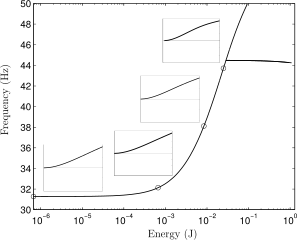
\includegraphics[width=\linewidth]{nlbeam/nnm/nnm1.pdf}
    \caption{}
  \end{subfigure}
  ~
  \begin{subfigure}[b]{0.45\textwidth}
    
\includegraphics[width=\linewidth]{nlbeam/nnm/nnm2.pdf}
    \caption{}
  \end{subfigure}
  \caption{Frequency-energy plot(FEP) of the
    \textbf{(a)} first- and
    \textbf{(b)} second NNM. Inserts show the NNM shapes (displacements of the
    main beam) for different energy levels.}
  \label{fig:nlbeam_nnm}
\end{figure}

Finally, the NNM backbone traces the lotus as seen in fig.
\ref{fig:nlbeam_sweep}.

\begin{figure}[!ht]
  \centering
  \includegraphics[width=0.6\textwidth]{nlbeam/hb/nfrc.pdf}
  \caption{
    % \textbf{(left)}:
    NFRC for forcing amplitudes (1,2,3,4)N from HB. The dashed line is
    the backbone of the first NNM and tracks the lotus;
    % \textbf{(right)}:
    % Phase lag wrt. the excitation force.;
    % Shown for the tip of the main beam.
    $\square$ denote $F=4N$.
    }
  \label{fig:nlbeam_sweep}
\end{figure}


\FloatBarrier
\section{System with clearences}
\label{sec:syst-with-clear}

A single DOF model with two clearances is simulated to obtain data for
characterisation with WT and RFS and estimation with FNSI. The model is only
briefly introduced below and the section is not intended to be a complete or
thorough derivation; as the interesting part is not the model, but applications
of the methods treated in this thesis.
Only changes in stiffness during impact is considered, ie. impact damping as
given by some impact models is ignored

\subsection{Model}

The model is a clamped-free beam with a pair of elastic stops at the free end
with optionally asymmetrical clearance distances $a_\pm$, see fig
\ref{fig:clear_schematic}.


\begin{figure}[!ht]
  \centering
  \centering
  \def\svgwidth{10cm}
  \import{fig/contact/}{beam.pdf_tex}
  \caption{Beam with elastic stops}
  \label{fig:clear_schematic}
\end{figure}


The bending vibrations of the beam are given by
\begin{equation}
  \label{eq:clear_EOM}
  \rho A \frac{\p^2 u(z,t)}{\p t^2} + \frac{\p^2}{\p z^2}
  \left( EI \frac{\p^2 u(z,t)}{\p z^2}  \right) +
  f_{res}(u(z_b,t)) \delta (z-z_b) +
  P_0 \sin(\Omega t) \delta(z-z_f)= 0
\end{equation}
where $EI, \rho, A, \delta(z), Q_0, u(z,t)$ denotes the bending stiffness, mass
density, cross section area, Dirac delta function, forcing amplitude and
relative transverse displacement, respectively, for the assumed uniform beam.
The forces are assumed point loads, where the external force act in $z_f$ and the
vibro-impact force at the impact location $z_b$ is given by

\begin{equation}
  \label{eq:clear_vibro_force}
  f_{res}(u) =
  \begin{cases}
    k_+(u - a_+) & u \geq a_+ \\
    0 &  a_+ > u > a_- \\
    k_-(u - a_+) & u \leq - a_- \\
  \end{cases}
\end{equation}
where $a_\pm$ are the clearance distances and $k_\pm$ the associated
stiffness's. Thus the stops behaves as one-sided springs.

The left end is clamped, giving the boundary conditions
\begin{equation}
  u(0,t) = 0, \quad u_z(0,t) = 0
\end{equation}
and at the right end, between stops, the beam moves freely giving a moment-
and transverse stress free condition
\begin{equation}
 a_+ > u > a_-: \quad u_{zz}(L,t) = 0, \quad u_{zzz}(L,t) = 0
\end{equation}

When the elastic stops are hit, the stress $\sigma = EIu_{zzz}$ is no longer
zero
\begin{equation}
  a_+ < u, u < a_-: \quad \sigma(z_b,t) = - f_{res}(u)
\end{equation}
Notice that the stress is opposite in direction to the displacement. For $k_\pm
\to \infty$, the stops are rigid and velocity changes sign instantly at each
impact, known as the Signorini nonpenetration condition.


An approximate solution to \eqref{eq:clear_EOM} is given by the modal expansion
\begin{equation}
  \label{eq:clear_modal}
  u_n(z,t) = \sum_{i=1}^n \phi_i(z) q_i(t)
\end{equation}
where $\phi_i$ is the mode shape satisfying the stated essential boundary
conditions and related to the $i$'th natural frequency
$\omega_i$; together they define the $i$'th mode for linear system of eq.
\eqref{eq:clear_EOM}, ie. with $f_{res}(u) = 0$.

The modal components $q_i(t)$ satifies the coupled nonlinear differential
equation
\begin{equation}
  \ddot q_i(t) + 2 \xi \omega_i \dot q_i(t) + \omega_i^2 q_i(t) +
  \frac{\phi_i(z_b)}{\rho A L} f_{res}(u_n(z_b,t)) +
  \frac{\phi_i(z_f) }{\rho A L}Q_0\sin(\Omega t)
  = 0, \quad
  i=1,...,n
\label{eq:clear_mode_expansion}
\end{equation}
where viscous damping have been added to account for dissipative effects.
This is not easily solved. The preprint by Rebouças~\autocite{reboucas2017a}
list different techniques for solving vibro-impact models as well as an example
of a thorough derivation of the nondimensionalized EOMs(though for a
parametrically excited vibro-impact).

\subsubsection{Numerical solution}

When eq. \eqref{eq:clear_modal} is driven around its first resonance, the higher
order modes ($i\geq 2$) are expected to have low influence as they are
increasingly damped. Thus a single-mode expansion can be used, as long as the
driving frequency is kept well below the second resonance.

Solving the system using Newmarks method, requires the derivatives of the
restoring force to be continuous. \autocite{kim2003a} list different smoothening
functions and the smoothening effect on the nonlinear response.
However I prefer using local regularisation with Hermite polynomials in the
interval $[a-\Delta, a+\Delta]$, where $2\Delta$ is the size of the
regularisation interval. Figure \ref{fig:fnl_piecewise} shows an example of a
regularised tri-linear restoring force; the purely linear behaviour of the
restoring force outside the regularisation interval is kept, which is why this
approach is favoured. \autocite{kim2003a} ensures continuity by changing the
piecewise linear functions to trigonometric functions.

\begin{figure}[!ht]
  \centering
  \def\svgwidth{10cm}
  \import{fig/contact/}{piecewise_linear.pdf_tex}
  \caption{Example of piecewise-linear restoring force. The insert image shows a
    closeup of the effect of the regularization $\Delta$.}
  \label{fig:fnl_piecewise}
\end{figure}


A regularised trilinear model for stiffness' $k_-, k, k_+$ and clearances $a_-,
a_+$ is given by, %\autocite{renson2014_phd}
\begin{equation}
  \label{eq:fnl_piecewise}
  f_{nl}(x) =
  \begin{cases}
    ka_+ + k_+(x-a_+) & x \geq a_+ + \Delta_+ \\
    p_+(t(x)) & a_+ + \Delta_+ > x > a_+ - \Delta_+ \\
    kx & a_+ - \Delta_+ \geq x \geq  -(a_- - \Delta_-) \\
    p_-(t(x)) & -(a_- + \Delta_-) > x > -(a_- + \Delta_-) \\
    ka_- + k_-(x-a_-) & x \leq -(a_- + \Delta_-) \\
  \end{cases}
\end{equation}
where $x$ is the relative distance between the two DOFs defining the nonlinear
connections, ie. the displacement for the single mode expansion.

The Hermite polynomials $p_\pm$ are defined as
\begin{equation}
  \label{eq:fnl_herm_pol}
  p_\pm(t) = h_{00}(t)p_k + h_{10}(t)(x_{k+1}-x_k)m_k + h_{01}(t)p_{k+1} + h_{11}(t)(x_{k+1} - x_k)m_{k+1}
\end{equation}
where $p_k$ and $p_{k+1}$ are the values of the restoring force at points $x_k =
a_\pm - \Delta$ and $x_{k+1} = a_\pm + \Delta$, respectively. $m_k$
and $m_{k+1}$ are the values of the restoring force derivative at the same $x_k$
and $x_{k+1}$ points; they correspond to the stiffness coefficients k and
$k_\pm$. The normalised displacement $t$ (termed the \textit{local scaled
  abscissa}) and $h_{ij}$ functions are

\begin{equation}
  \label{eq:fnl_piecewise_coeff}
  \begin{gathered}
    t(x) = \frac{x - x_k}{x_{k+1} - x_k}\\
    h_{00}(t) =  2t^3 - 3t^2 + 1, \quad
    h_{10}(t) = t^3 - 2t^2 + t \\
    h_{01} = -2t^3 + 3t^2, \quad
    h_{11} = t^3 - t^2 \\
  \end{gathered}
\end{equation}

It should be noted that numerically solving systems with a large difference in
stiffness(\textit{stiff} systems) might not be easy. When the
beam hit the stops, some spurious high frequencies might appear in the numerical
solution. These spurious frequencies may disappear by choosing a smaller
time-step and if not, the solutions becomes unstable. In that case a time
integration method with numerical damping should be used. A possibility is to
use a Newmark scheme with $\gamma > \frac{1}{2}$ in order to introduce some
numerical damping. Unfortunately this scheme is only of first order convergence
and the effect of the damping can affect amplitude of the solution. Preferable
another scheme should be used, see appendix \ref{sec:newmark_summary} for at bit
more on the Newmark method and references to alternatives.

As a single mode model is used, an easier approach is to use a stiff first order ODE
solver, eg. a \textit{Radau}-type. Then either event-detection for impacts or the
reformulation of the piecewise function \eqref{eq:clear_vibro_force} into

\begin{equation}
  \label{eq:clear_oneline}
  f_{res}(u) = u + (1-\alpha)\frac{|u-a|-|u+a}{2}
\end{equation}
which is valid for symmetric stops $a = a_+=a_-$ could be used. $||$ is the
absolute value and $\alpha \leq 1$ is the slope in-between the stops, ie. 0. The
slope of \eqref{eq:clear_oneline} is one after impact. To get stiffer impacts
$f_{res}$ is simply multiplied by a desired factor. The latter reformulation
should be preferred as long as the time steps are not too large, which could
correspond to a large penetration of the stop \footnote{For solving ODEs
  \autocite{pydstool} is recommended. The system is automatically compiled into
  c-code, along with any event-detection. As a result, simulation is ten-fold
  faster than what can be achieved by matlab.}.



\subsection{Identification}
\label{sec:contact_identification}

The one-mode approximation
\begin{equation}
  \label{eq:one_mode}
  \ddot x + 2 \xi \omega \dot x + \omega^2x + 3f_{res}(x) = q\sin(\omega_t t)
\end{equation}
with symmetrical stops $a= 0.1745$, $\omega^2 = 1$, $\xi=0.025$, $q = 0.03$ and
$f_{res}$ given by \eqref{eq:clear_oneline} is used. The factor 3 controls the
impact stiffness.


\subsubsection{Characterisation}

The system \eqref{eq:one_mode} is excited by a linear sine sweep from
$\omega_t=[0.001,2]$rad/s with a sweep rate of $0.01$Hz/min.

Figure shows the time series for a forward sweep and the NFRC calculated by HB.
For HB the general model for $f_{res}$ \eqref{eq:fnl_piecewise} is used, as the
derivative of the restoring force is needed.
A stiffening effect is seen, which is explained by the constraining effects of the
stops. When the energy is increased, the stiffer stops prevents the amplitude
from increasing proportionally and the system responds by increased
frequency.

\begin{figure}
  \centering
  \includegraphics[width=0.6\textwidth]{contact/nfrc.pdf}
  \caption{Forward sweep and HB for system \eqref{eq:one_mode}. Sweep rate:
    0.01Hz/min and $q=0.03$. Dashed line indicates a unstable periodic solution.}
  \label{fig:contact_nfrc}
\end{figure}


Figure \ref{fig:contact_characterisation}(a) shows the wavelet transform, where
uneven higher harmonics are seen. The magnitude and number of the higher
harmonics are controlled by the impact duration, ie. a short impact, or rapid
change in velocity, results in more harmonics as the impact resembles a narrower
impulse with a broader frequency content.

Figure \ref{fig:contact_characterisation}(b) shows the restoring force and is
clearly piecewise linear. The vertical dashed lines indicate the stops and the
clearance distance can be determined quite accurate from the plot.

\begin{figure}
  \centering
  \begin{subfigure}[b]{0.45\textwidth}
    \includegraphics[width=\linewidth, height=6cm]{contact/wt.png}
    \caption{}
  \end{subfigure}
  ~
  \begin{subfigure}[b]{0.45\textwidth}
    \includegraphics[width=\linewidth, height=6cm]{contact/rfs.tikz}
    \caption{}
  \end{subfigure}
  \caption{Characterisation of system \eqref{eq:one_mode} using a forward sine sweep.
    \textbf{(a)}: Wavelet transform;
    \textbf{(b)}: Restoring force surface slice showing the restoring force.
    Dashed lines shows the location of the stops.}
  \label{fig:contact_characterisation}
\end{figure}



\subsubsection{Estimation}

The estimation of the of the system \eqref{eq:one_mode} is done by FNSI using
cubic splines as basis functions.

\paragraph{Spline formulation}

To resemble a linear piecewise function, a polynomial of sufficiently high order
can be used. But as stated, high order polynomials shows oscillations around
origin. Instead piecewise cubic polynomials (splines) are used, as introduced in
\autocite{noel2014b}. Spline formulations are found in the handbook
\autocite{boor2001a}.

To find the cubic spline representation of the nonlinear force $f(x)$, let $x$
be divided into $R$ segments of arbitrary length defined by their abscissas
$x_k$ for $k=1,...,R+1$. Each abscissa is associated with a ordinate $f_k$;
together they define a knot $(x_k, f_k)$.

Thus for the displacement $x$ between knots $k$ and $k+1$, the corresponding
spline approximation of $f$ is given by

\begin{equation}
  \label{eq:spline_interp}
  \begin{aligned}
    f(x) =& (2t^3-3t^2+1)x_k + (-2t^3+3t^2)x_{k+1} + \\
    &(t^3-2t^2+t)(x_{k+1}-x_k)x'_k + (t^3-t^2)(x_{k+1}-x_k)x'_{k+1}
  \end{aligned}
\end{equation}
where $t$ is the normalised displacement. To calculate the first order
derivatives $x'_k = \frac{\p x_k}{\p x}$, $R+1$ constraints are needed.
Forcing the cubic splines and the first two derivatives to be continuous across
each interior knot gives $R-1$ constraints:

\begin{equation}
  \label{eq:spline_contraint1}
  \begin{aligned}
    \frac{x'_{k-}}{x_k-x_{k-1}} + 2 \left( \frac{1}{x_k-x_{k-1}} +
      \frac{1}{x_{k+1}-x_{k}} \right) x'_k + \frac{x'_{k+1}}{x_{k+1}-x_k} = \\
    3
    \left( \frac{x_k-x_{k-1}}{(x_k-x_{k-1})^2} +
      \frac{x_{k+1}-x_{k}}{(x_{k+1}-x_{k})^2} \right)
  \end{aligned}
\end{equation}

As the nonlinear force is required to be nonlinearizable, ie. is zero and have
zero slope at equilibrium, this is also enforced for the segment containing the
equilibrium point, giving the last two constraints. This is generally called the
boundary condition for generic spline interpolation.

\begin{align}
  \label{eq:spline_constraint2}
  \begin{aligned}
    (t_0^3 -2t_0^2 +t_0)(x_{k+1} - x_k)x'_k +
    (t_0^3-t_0^2)(x_{k+1} - x_k)x'_{k+1} = \\
    -(2t_0^3-3t_0^2+1)x_k -
    (-2t_0^3 +3t_0^2)x_{k+1}
  \end{aligned}\\
  \begin{aligned}
    (3t_0^2 -4t_0 +1)(x_{k+1} - x_k)x'_k +
    (3t_0^2-2t_0)(x_{k+1} - x_k)x'_{k+1} = \\
    6(t_0-t_0^2)(x_k + x_{k+1})
  \end{aligned}
  \label{eq:spline_contraint3}
\end{align}
where $t_0 = \frac{-x_k}{x_{k+1}-x_k}$.

Thus to summarise:
Given the displacements $\bm x$ and knot placements $x_k$, the linear constraint
equations \eqref{eq:spline_contraint1}-\eqref{eq:spline_contraint3} are
solved(as a tridiagonal system) and used to find the basis function from eq.
\eqref{eq:spline_interp}.
The number of knots and their abscissas($x_k$) should ideally be chosen by minimising
the difference in some metric between the predictions of the nonlinear model and
measured data. In reality it is still done by trial and error. In the current
implementation the abscissas are distributed so the segments are divided into
equal lengths.

\paragraph{Results}

Using a low and high level multisine excitation's with RMS values of $0.005$ and
$0.2$, the identified linear parameters are seen in table \ref{tab:contact_par}.
At low level, where the stops are not activated, the expected linear parameters
are obtained to high precision. At high level, without nonlinear basis
functions, an increased natural frequency is obtained. Using the cubic splines,
the correct linear frequency is obtained whereas the damping is estimated too
low.

\begin{center}
\resizebox{\columnwidth}{!}{%
  \begin{tabular}{@{} l *{4}{c} @{}}
    \hline
    & Mode & Frequency (rad/s) & Damping ration (\%) & Deviation from linear freq. (\%) \\
    \hline
    \tiny{Low}  &1 & 1  & 2.5 \\
    \hline
    \tiny{High, lin} &1 & 1.15 & 1.0  & 14.8 \\
    \hline
    \tiny{High, nonlin} &1 & 0.995 & 1.6 & 0.5 \\
    \hline
  \end{tabular}
  }
  \captionof{table}{Estimated linear natural frequencies and damping ratios for
    the system \eqref{eq:one_mode} .
    \textbf{(upper)}: Low level, linear identification;
    \textbf{(middle)}: High level, linear identification;
    \textbf{(lower)}: High level, nonlinear identification.
  }
  \label{tab:contact_par}
\end{center}


Comparing the estimated nonlinear restoring force by the cubic splines to the
exact in fig. \ref{fig:contact_rf}, it is seen FNSI is able to capture the
discontinuity using splines. 15 spline segments are specified for estimation,
giving 16 basis functions(one for each knot ordinate). The high number of
splines is chosen to show that FNSI is able to estimate many parameters.
It have not been investigated why the damping estimation is wrong or if
tweaking the number of splines would result in a better estimate.

Is is however expected that FNSI gives better estimates for natural frequencies
than damping, as discussed in sec. \ref{sec:fnsi-estimation-error}.

\begin{figure}
  \centering
  \includegraphics[width=0.8\textwidth, height=8cm]{contact/rf}
  \caption{
    Nonlinear restoring force for the system \eqref{eq:one_mode}.
    \sampleline{}: Restoring force from splines estimation. Markers show knot locations;
    \textcolor{blue}{\sampleline{dashed}}: Analytical restoring force
  }
  \label{fig:contact_rf}
\end{figure}





\FloatBarrier


%%% Local Variables:
%%% mode: latex
%%% TeX-master: "../report"
%%% End:
